\chapterimage{images/fragments/fragments.jpg} % Chapter heading image

\chapter{Fragments}
Fragments are an optional layer you can put between your activities and your widgets, designed to help you reconfigure your activities to support screens both large (e.g., tablets) and small (e.g., phones). 

If you regard Android as an MVC architecture, fragments and activities combine to be the controller layer. Fragments serve as a local controller, focused on their set of widgets, populating them from model data, and handling
their events. Activities will serve as more of an orchestration layer, handling cross- fragment communications (e.g., a click in Fragment A needs to cause a change in what is displayed in Fragment B).

This chapter is built from the following resources: \cite{Point2017, TueDao2017, Guide2017, murphymarkl.2017,Gleason2017}.

\section{Design Philopsophy of fragments}
Android introduced fragments in Android 3.0 (API level 11), primarily to support more dynamic and flexible UI designs on large screens, such as tablets. Because a tablet's screen is much larger than that of a handset, there's more room to combine and interchange UI components. Fragments allow such designs without the need for you to manage complex changes to the view hierarchy. By dividing the layout of an activity into fragments, you become able to modify the activity's appearance at runtime and preserve those changes in a back stack that's managed by the activity.

Fragments offer

\begin{itemize}
	\item Modularity: Dividing complex activity code across fragments for better organization and maintenance.
	\item Reusability: Placing behavior or UI parts into fragments that can be shared across multiple activities.
	\item Adaptability: Representing sections of a UI as different fragments and utilizing different layouts depending on screen orientation and size.
\end{itemize}

You should design each fragment as a modular and reusable activity component. That is, because each fragment defines its own layout and its own behaviour with its own life cycle callbacks, you can include one fragment in multiple activities, so you should design for reuse and \textbf{avoid directly manipulating one fragment from another fragment}. This is especially important because a modular fragment allows you to change your fragment combinations for different screen sizes.

\begin{figure}
	\centering
	\includegraphics[width=0.7\textwidth]{images/fragments/framgentswhy.png}
	\label{fig:whyfragments}
	\caption{You should design each fragment as a modular, adaptable and reusable component.}
\end{figure}

\section{How to work with activities and fragments - Dual Panze}
\begin{framed}
	The source code which accompanies this chapter can be found on the following link: \url{https://github.com/eothein/rage_against_the_app}. It is an an adaptatjon of the project from \cite{Gleason2017a}

\end{framed}

To create a fragment, you must create a subclass of Fragment (or an existing subclass of it). The Fragment class has code that looks a lot like an Activity. It contains callback methods similar to an activity, such as onCreate(), onStart(), onPause(), and onStop(). In fact, if you're converting an existing Android application to use fragments, you might simply move code from your activity's callback methods into the respective callback methods of your fragment.

\begin{figure}
	\centering
	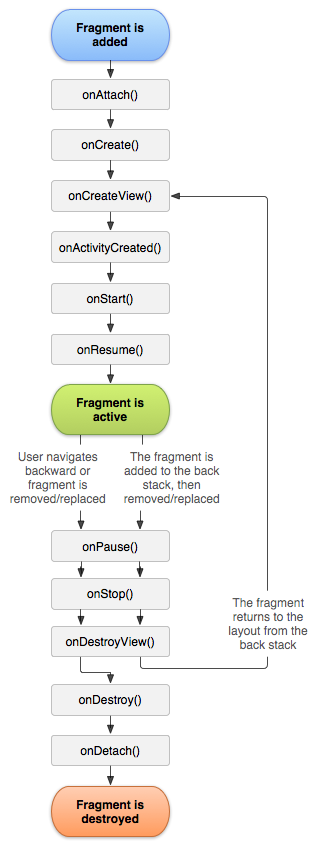
\includegraphics[width=0.5\textwidth]{images/fragments/lifecycle.png}
	\label{fig:fragcycle}
	\caption{The lifecycle of a fragment (while its activity is running).}
\end{figure}
Managing the lifecycle of a fragment is a lot like managing the lifecycle of an activity. Like an activity, a fragment can exist in three states:
\begin{description}
	\item[Resumed] The fragment is visible in the running activity.
	\item[Paused] Another activity is in the foreground and has focus, but the activity in which this fragment lives is still visible (the foreground activity is partially transparent or doesn't cover the entire screen).
	\item[Stopped] The fragment isn't visible. Either the host activity has been stopped or the fragment has been removed from the activity but added to the back stack. A stopped fragment is still alive (all state and member information is retained by the system). However, it is no longer visible to the user and is killed if the activity is killed.
\end{description}


\subsection{Creating a Fragment}
In Kotlin you delcare a Fragment by extending the Fragment class. 
\lstinputlisting[firstline=18,lastline=42	,language=Kotlin, caption={Creating a Fragment}, label=code:fragment]{srccode/fragments//RagecomicDetailFragment.kt}

This is what this code does:
\begin{enumerate}
	\item Declares RageComicDetailsFragment as a subclass of Fragment.
	\item An onCreate method which initialises the dependencies and or restores the state
\end{enumerate}

In most cases you need the following methods in order for a Fragment to work.

\begin{itemize}
	\item onCreate()
	The system calls this when creating the fragment. Within your implementation, you should initialize essential components of the fragment that you want to retain when the fragment is paused or stopped, then resumed.
	\item onCreateView()
	The system calls this when it's time for the fragment to draw its user interface for the first time. To draw a UI for your fragment, you must return a View from this method that is the root of your fragment's layout. You can return null if the fragment does not provide a UI.
	\item onPause()
	The system calls this method as the first indication that the user is leaving the fragment (though it doesn't always mean the fragment is being destroyed). This is usually where you should commit any changes that should be persisted beyond the current user session (because the user might not come back).
\end{itemize}
Also like an activity, you can preserve the UI state of a fragment across configuration changes and process death using a combination of onSaveInstanceState(Bundle), ViewModel, and persistent local storage. 

The most significant difference in lifecycle between an activity and a fragment is how one is stored in its respective back stack. An activity is placed into a back stack of activities that's managed by the system when it's stopped, by default (so that the user can navigate back to it with the Back button, as discussed in Tasks and Back Stack). However, a fragment is placed into a back stack managed by the host activity only when you explicitly request that the instance be saved by calling addToBackStack() during a transaction that removes the fragment.

\subsection{Adding a Fragment to an Activity}

Adding the fragment to an activity can either be done by declaring it in the XML layout file of the activity, or dynamically in the code by using FragmentTransactions.

\subsubsection{Adding a Fragment Dynamically}
First, you grab the FragmentManager by referencing supportFragmentManager.

Then, you ask that FragmentManager to start a new transaction by calling beginTransaction(). Next, you specify the add operation that you want by calling add and passing in:

\begin{enumerate}
\item The view ID of a container for the fragment’s view hierarchy in the activity’s layout. If you take a look at the layout you'll find single pane.
\item The fragment instance to be added.
\item A string that acts as a tag/identifier for the fragment instance. This allows the FragmentManager to later retrieve the fragment for you.
\end{enumerate}

You can also remove or replace fragments one by another. 

Finally, you ask the FragmentManager to execute the transaction by calling commit().

\lstinputlisting[firstline=137,lastline=140,language=Kotlin, caption={Replacing the fragment by using transactions.}, label=code:fragmentCode]{srccode/fragments/RagecomicListActivity.kt}

Of course your layout file should have a place holder for your Fragment.

\lstinputlisting[firstline=33,lastline=37,language=XML, caption={The XML layout file for an activity with a dynamic Fragment. The Framelayout servers as a place holder}, label=code:dynamicFragment]{srccode/fragments/layout-w900dp/ragecomic_list.xml}

As seen above, managing fragments in your activity requires the FragmentManager. 

Some things that you can do with FragmentManager include:

\begin{enumerate}
	\item Get fragments that exist in the activity, with findFragmentById() (for fragments that provide a UI in the activity layout) or \item findFragmentByTag() (for fragments that do or don't provide a UI).
	\item Pop fragments off the back stack, with popBackStack() (simulating a Back command by the user).
	\item Register a listener for changes to the back stack, with addOnBackStackChangedListener().
\end{enumerate}

\subsection{Communicating with the Activity}
You can  define a callback interface inside the fragment and require that the host activity implement it. When the activity receives a callback through the interface, it can share the information with other fragments in the layout as necessary.





